\clearpage

\lehead[]{\normalfont\sffamily\hspace*{-2.00cm}\textcolor{white}{\colorbox{lightblue}{\parbox[c][0.70cm][b]{1.60cm}{
\makebox[1.60cm][r]{\thechapter}\\ \makebox[1.60cm][r]{ÜBUNG}}}}\hspace{0.17cm}\textcolor{lightblue}{\chaptertitle}}
\rohead[]{\textcolor{lightblue}{\chaptertitle}\normalfont\sffamily\hspace*{0.17cm}\textcolor{white}{\colorbox{lightblue}{\makebox[1.60cm][l]{\thechapter}}}\hspace{-2.00cm}}
%\chead[]{}
\rehead[]{\textcolor{lightblue}{AvHG, Inf, My}}
\lohead[]{\textcolor{lightblue}{AvHG, Inf, My}}

\section{Übungsaufgaben: Client/Server}

\subsection{Aufgabe 1: Echo-Client \tagLK}
\noindent \emph{Neue Sprachmittel: Netzwerkverbindung mit \texttt{Socket(host, port)} aufbauen, Datenstrom mit \texttt{InputStreamReader} (\texttt{"UTF-8"}) zeichenweise bis \texttt{-1} einlesen. (Eignet sich bereits als direkter Vorgriff nach Kapitel~\ref{chap:dateizugriffe}.) Bidirektionale Kommunikation (\texttt{OutputStreamWriter}, \texttt{write()}, \texttt{flush()}, \texttt{System.lineSeparator()}), eigener Lese-Thread (\texttt{extends Thread}) und sauberes Trennen der Verbindung. (Eignet sich bereits als direkter Vorgriff nach Kapitel~\ref{chap:dateizugriffe}.)}

Im Kurs-Repository findest du die ausführbare JAR-Datei
\myFile{EchoServer.jar}. Wenn du diese startest, läuft der Server auf Port
\lstinline|22222|. Der Echo-Server sendet alle Daten, die an ihn geschickt
werden, wieder an den Absender zurück. Schreibe einen Client, der eine
Verbindung zum Echo-Server aufbaut. Der Benutzer kann den Namen des Servers
eingeben. Nachdem die Verbindung erfolgreich aufgebaut wurde, kann der Benutzer
in einem Textfeld Sätze eintippen. Sobald er auf den danebenstehenden Button
drückt, wird die eingegebene Zeile an den Server gesendet. Wenn eine Verbindung
aufgebaut wird, wird für das Einlesen der Daten, die der Server zurücksendet,
ein eigener Thread erzeugt. Dieser Lese-Thread schreibt die empfangenen Daten
in eine \myClass{JTextArea} (eingebettet in eine \myClass{JScrollPane}) des
Anwendungsfensters. Die Verbindung zum Echo-Server kann über
einen Button getrennt werden. Wenn der Client die Verbindung beendet, schließt
auch der Server die Verbindung. Der Lese-Thread erhält nach dem Schließen der
Verbindung durch den Server eine \myClass{IOException}. Wenn er eine
\myClass{IOException} erhält, soll sich der Lese-Thread selbstständig beenden.
Dies überprüft man am besten durch eine Ausgabe auf der Konsole.

\begin{center}
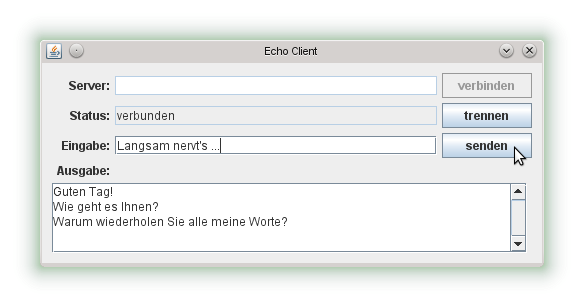
\includegraphics[width=0.75\textwidth]{./inf/SEKII/45_Java_ClientServer/EchoClient.png}
\end{center}

\subsubsection{Tipp: Zeilenumbrüche}

Wenn man in der \myClass{JTextArea} eine neue Zeile anfangen möchte, kann man
dies kodieren, indem man nacheinander die Zeichen \emph{Carriage Return}
(Wagenrücklauf, ASCII-Zeichen Nr.\ $13$) und \emph{Line Feed} (Zeilenvorschub,
ASCII-Zeichen Nr.\ $10$) sendet. Man kann entweder die ASCII-Zeichen als
Integer-Werte senden oder sie mithilfe einer Escape-Sequenz in einem String
kodieren. Beispiel für die Kodierung eines Zeilenumbruchs in einem String:

\begin{lstlisting}
String text = "Erste Zeile\r\nZweite Zeile.";
\end{lstlisting}

\lstinline|\r| steht für Carriage Return

\lstinline|\n| steht für Line Feed

Sinnvoll ist, dass der EchoClient beim Senden eines Strings an den Server
automatisch einen Zeilenumbruch an den Text des Benutzers anfügt.

\textbf{Allerdings werden Zeilenumbrüche je nach verwendetem Betriebssystem
unterschiedlich kodiert (\lstinline|\r\n| ist richtig für Windows).
Sinnvoller ist es deshalb, die statische Methode
\lstinline|System.lineSeparator()| zu benutzen. Sie erzeugt je nach verwendetem
Betriebssystem die richtige Zeichenfolge}:

\begin{lstlisting}
String text = "Erste Zeile" + System.lineSeparator() + "Zweite Zeile.";
\end{lstlisting}


\subsection{Aufgabe 2: Echo-Server \tagLK}
\noindent \emph{Neue Sprachmittel: \texttt{ServerSocket(port)} und \texttt{accept()} in einem eigenen Hintergrund-Thread ausführen, damit die Swing-Oberfläche nicht blockiert. Parallele Bedienung mehrerer Clients (für jedes \texttt{accept()} einen eigenen Client-Thread mit übergebenem \texttt{Socket} starten).}

Programmiere einen Echo-Server, der alle Eingaben, die er von einem Client
erhält, wieder an den Client zurücksendet. Der Echo-Server soll mehrere
Clients parallel bedienen können. Wenn eine Client-Verbindung aufgebaut wurde,
generiert er für die Kommunikation mit dem Client einen eigenen Thread. Im
Konstruktor des Threads wird der Socket, der für diesen Client erzeugt wurde,
als Parameter übergeben. Der Thread beendet sich, wenn die Verbindung vonseiten
des Clients geschlossen wurde. Dies kann entweder durch eine Exception
angezeigt werden oder dadurch, dass der Server in der \lstinline|read()|-Methode
ein Byte mit dem Wert \lstinline|-1| erhält.


\subsection{Zusatzaufgabe: Chat-Client und -Server \tagZusatz}
\noindent \emph{Neue Sprachmittel: Dynamische Verwaltung verbundener Clients mit \texttt{ArrayList<OutputStreamWriter>}, Weiterleitung an alle Clients und Thread-Synchronisation mit einem Monitor (\texttt{synchronized}).}

\subsubsection{Client}

Der Benutzer des Chat-Clients kann die Adresse des Servers und einen
selbstgewählten Namen eingeben. Nachdem der Benutzer einen Button gedrückt hat, baut
der Chat-Client eine Verbindung zum Chat-Server auf. Zur Kommunikation wird der 
Port $13131$ verwendet.

Der Benutzer kann über ein Textfeld zeilenweise Text eingeben, der an den
Server gesendet wird und vom Server an alle anderen angemeldeten Clients
weitergeleitet wird. Der Client sendet zuerst den selbstgewählten Namen des Benutzers
(damit die anderen Benutzer wissen, wer den Text gesendet hat), dann folgen ein
oder mehrere Trennungszeichen und dahinter der vom Benutzer geschriebene Text,
der mit einem Zeilenumbruch (\lstinline|System.lineSeparator()|) endet:

\lstinline|Name: Text|

Im Frame gibt es neben dem Eingabefeld eine \myClass{JTextArea}, in der alle
gesendeten Texte angezeigt werden. Das Empfangen der Texte vom Server geschieht
in einem Hintergrund-Thread. Die Texte können unverändert in die
\myClass{JTextArea} eingetragen werden. Die durch den Aufruf von
\lstinline|System.lineSeparator()| erzeugten Steuerzeichen sorgen dafür, dass
nach jedem Text ein Zeilenumbruch erfolgt.

\subsubsection{Server}

Der Server ermöglicht es einer beliebigen Anzahl von Clients, miteinander zu
kommunizieren. In einem Textfeld zeigt er die Anzahl der Clients an, die
momentan mit dem Server verbunden sind. Zur Verwaltung der Clients besitzt der
Server außerdem eine Liste aller \myClass{OutputStreamWriter} der
angeschlossenen Clients, die mit der Klasse \myClass{ArrayList} verwaltet wird.

Der Server erzeugt in einem speziellen Thread seinen Haupt-Socket (mit der
vereinbarten Portnummer), auf dem er auf eingehende Verbindungen wartet. Wenn
ein neuer Client \glqq anruft\grqq , holt er sich den
\myClass{OutputStreamWriter} für die neue Client-Verbindung und trägt ihn in
die Liste der \myClass{OutputStreamWriter} ein. Dann generiert er einen eigenen
Thread für die neue Client-Verbindung. Im Konstruktor des Threads werden das
Anwendungsfenster sowie der \myClass{InputStreamReader} und
\myClass{OutputStreamWriter} dieses speziellen Clients übergeben.

Jeder Client-Thread wartet auf eingehende Texte von seinem Client. Ein Text
wird bis zum Zeilenumbruch eingelesen und anschließend in einer Schleife an
alle Clients geschrieben (auch an den, der den Text gesendet hat, damit auch
dieser den Text in seine \myClass{JTextArea} einträgt). Damit die Texte von zwei
verschiedenen Benutzern sich nicht vermischen, muss das Senden der Texte an
die Clients mit einem Monitor geschützt werden.

Wenn ein Client die Verbindung zum Server schließt, muss der für diesen Client
zuständige Thread den \myClass{OutputStreamWriter} des Clients aus der Liste der
\myClass{OutputStreamWriter}-Objekte löschen und die Anzeige der Clientanzahl im
Anwendungsfenster aktualisieren. Anschließend beendet sich der Client-Thread.

\subsubsection{Klasse \myClass{ArrayList}}

Mit der Klasse \myClass{ArrayList} kann man dynamische Listen verwalten. Der
Vorteil gegenüber der Verwendung von Arrays ist, dass die Klasse bei Bedarf
automatisch Speicherplatz für neue Objekte anlegt, und dass man Objekte aus der
Liste heraus löschen kann, ohne dass Lücken entstehen.

Benötigte Import-Anweisung:

\begin{lstlisting}
import java.util.ArrayList;
import java.util.List;
\end{lstlisting}

Anlegen einer \myClass{ArrayList}

Schema:

\begin{lstlisting}
List<Datentyp> variable = new ArrayList<>();
\end{lstlisting}

Beispiel:

\begin{lstlisting}
List<OutputStreamWriter> listOSW = new ArrayList<>();
\end{lstlisting}

Methoden (Auswahl):

\bgroup
\def\arraystretch{1.2}
\begin{tabularx}{\textwidth}{|p{65mm}|X|}
\hline
\textbf{Methode} &
\textbf{Beschreibung}
\\ \hline
\texttt{public boolean add(Datentyp o)} &
Hängt ein neues Objekt an die Liste an.
\\ \hline
\texttt{public boolean remove(Datentyp o)} &
Löscht das angegebene Objekt aus der Liste.
\\ \hline
\texttt{public void clear()} &
Löscht alle Objekte aus der Liste.
\\ \hline
\texttt{public int size()} &
Gibt an, wie viele Objekte sich in der Liste befinden.
\\ \hline
\texttt{public Datentyp get(int index)} &
Gibt das Element mit dem angegebenen Index zurück.
\\ \hline
\end{tabularx}
\egroup